\section{Protocole expérimental et résultats}

%%%%%%%%%%%%%%%%%%%%%%%%%%%%%%%%%%%%%%%


%\begin{frame}{Le simulateur}
%    \begin{figure}
%        \centering
%        \begin{tikzpicture}[scale=1, auto, >=stealth']
    \small

    % TikZ styles for drawing %%%%%%%%%%%%%%%%%%%%%%%%%%%%%%%%%%%%%%%%%%%%%%%%%%%%%%
    \tikzstyle{block} = [draw,rectangle,thick,minimum height=2em,minimum width=2em]
    \tikzstyle{rounded} = [draw,rectangle,rounded corners=2mm,thick,minimum height=2em,minimum width=2em]
    \tikzstyle{sum} = [draw,circle,inner sep=0mm,minimum size=2mm]
    \tikzstyle{connector} = [->,thick]
    \tikzstyle{line} = [thick]
    \tikzstyle{branch} = [circle,inner sep=0pt,minimum size=1mm,fill=black,draw=black]

    % Node placement with matrix library (3x5 array) %%%%%%%%%%%%%%%%%%%%%%%%%%%%%%%%%%%%
    \matrix[ampersand replacement=\&, row sep=0.2cm, column sep=0.5cm] {

      % row 1
      \node[branch, yshift=-2mm] (b2) {}; \&
      \node[block] (control) {Contrôleur}; \&
      \node[rounded] (noise) {Bruit}; \&
      \node[branch] (b3) {}; \&
      \node[block] (model) {Système mécanique (bras)};
      \\

      % row 2
      \&
      \node[sum] (kalman) {K}; \&
      \&
      \&
      \\

      % row 3
      \&
      \&
      \node[rounded] (delta) {Délai}; \&
      \&
      \node[branch] (b4) {};
      \\
    };

     % Now link the nodes %%%%%%%%%%%%%%%%%%%%%%%%%%%%%%%%%%%%%%%%%%%%%%%%%%%%%%%%%%%%%%%%
     \draw [line]      ($(control.west) + (-1cm, 2mm)$) -- ($(control.west) + (-1cm, 2mm)$) node[left] {$\jstate^*$};
     \draw [line]      (b2) -- ($(control.west) + (-1cm, -2mm)$) node[left] {$\jstate_0$};
     \draw [connector] ($(control.west) + (-1cm, 2mm)$) -- ($(control.west) + (0, 2mm)$);
     \draw [connector] (b2) -- ($(control.west) + (0, -2mm)$);
     \draw [connector] (control) -- node {$\jctrl$} (noise);
     \draw [line]      (noise) -- node {$\tilde{\jctrl}$} (b3);
     \draw [connector] (b3) -- (model);
     \draw [connector] (b3) |- (kalman);
     \draw [line]      (model) -- node {$\jstate_{t+1}$} (b4);
%     \draw [connector] (b4) -- ++(2.5cm,0) -- ++(0,3cm) -- ++(-2.5cm,0) -- node {$\jstate_t$} (model.north);
     \draw [connector] (b4) -- (delta);
     \draw [connector] (delta) -| (kalman);
     \draw [line]      (kalman) -| node[pos=0.20] {$\tilde{\jstate}$} (b2);

\end{tikzpicture}

%    \end{figure}
%\end{frame}

%%%%%%%%%%%%%%%%%%%%%%%%%%%%%%%%%%%%%%%

\subsection{}

\begin{frame}{Les expériences}
    \begin{block}{Motivations}
        Est-ce que le découpage du problème initial permet de conserver les propriétés intéressantes de QOPS~:
        \begin{itemize}
            \item efficacité~: trouver le \og{}meilleur\fg{} mouvement~?
            \item réalisme~: vérifier les mêmes principes clés
            \begin{itemize}
                \item la {\em minimisation de la variance au point final} $[$Harris et Wolpert 98$]$
                \item le {\em principe d'intervention minimum} $[$Todorov et Jordan 02$]$
%                \item relation durée du mouvement/amplitude
%                \item anisotropie
%                \item loi de Fitts
%                \item profil de variabilité
            \end{itemize}
        \end{itemize}
    \end{block}
    Tout en réduisant le temps de calcul~?
\end{frame}

\begin{frame}{Le système mécanique utilisé}
    Modèle tiré de $[$Li 2008$]$ et $[$Rigoux et Guigon 11$]$
    \begin{figure}
        \centering
        \subfigure{\includegraphics[width=.47\linewidth]{fig/arm2_fr}}~~~
        \subfigure{\includegraphics[width=.47\linewidth]{fig/muscles_fr}}
    \end{figure}
    Modèle mécanique simple (motivations techniques)
\end{frame}

\begin{frame}{Performances du contrôleur}
    \begin{itemize}
        \item Comparer QOPS $[$Rigoux et Guigon 11$]$ et $\qopslqp$
        \begin{itemize}
            \item Coût des solutions~: $\costfuntionhat\left(\jctrl_{\{0..t_f\}}\right) = \sum \jctrl_t^2$
            \item Vitesse d'exécution
        \end{itemize}
    \end{itemize}
    \begin{columns}
        \begin{column}{0.60\textwidth}
            \begin{center}
                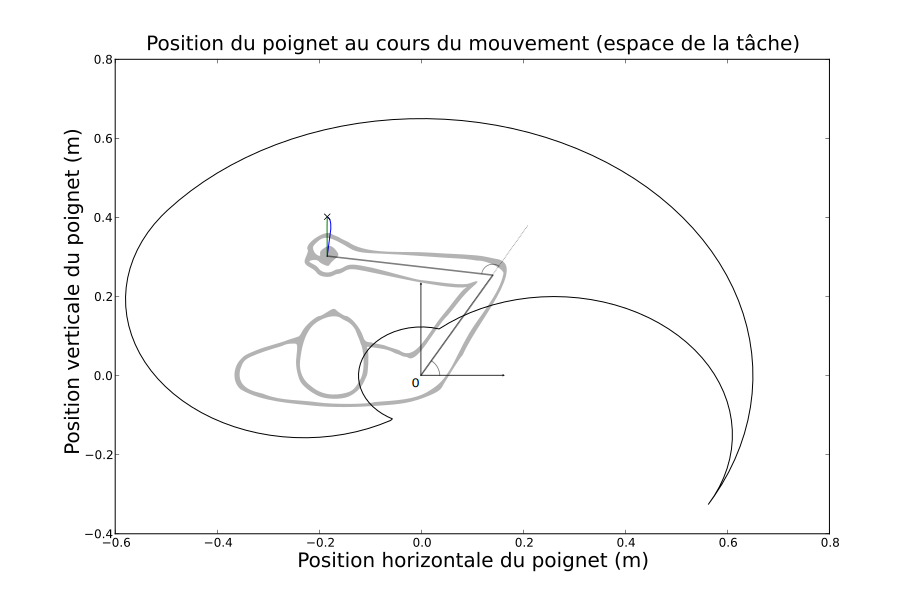
\includegraphics[width=.95\linewidth]{fig/cost_2}
            \end{center}
        \end{column}
        \begin{column}{0.40\textwidth}
            \begin{block}{Résultats}
                \begin{itemize}
                    \item Coût~: +40\%
                    \item Temps de calcul divisé par 3
                \end{itemize}
            \end{block}
        \end{column}
    \end{columns}
\end{frame}

%\begin{frame}{Relation amplitude/durée du mouvement}
%    \begin{itemize}
%        \item Propriété observée par $[$Gordon et al. 94$]$
%        \item Relation linéaire entre la durée du mouvement et son amplitude
%    \end{itemize}
%    \begin{figure}
%        \centering
%        \subfigure{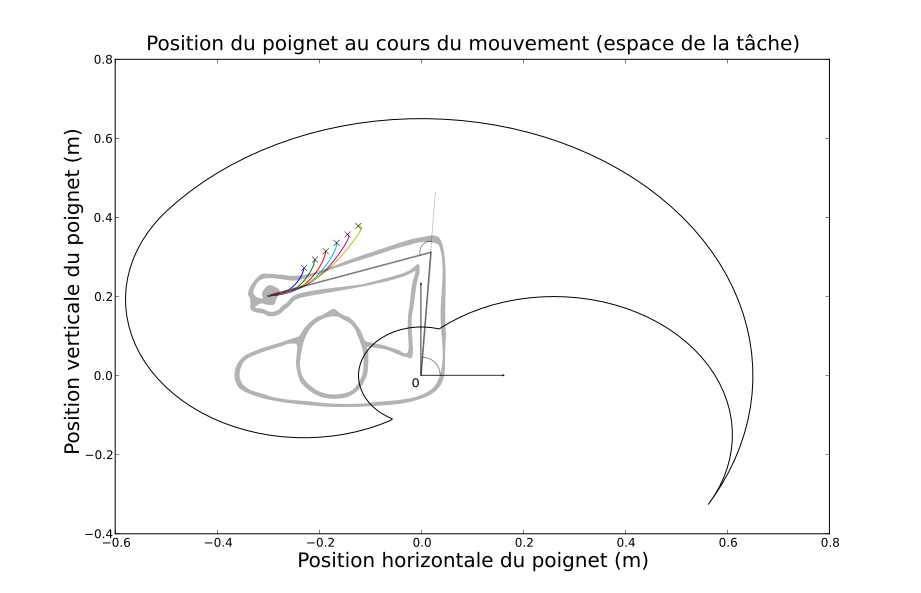
\includegraphics[width=.40\linewidth]{fig/lqp_scaling_paths_2}}~~~
%        \subfigure{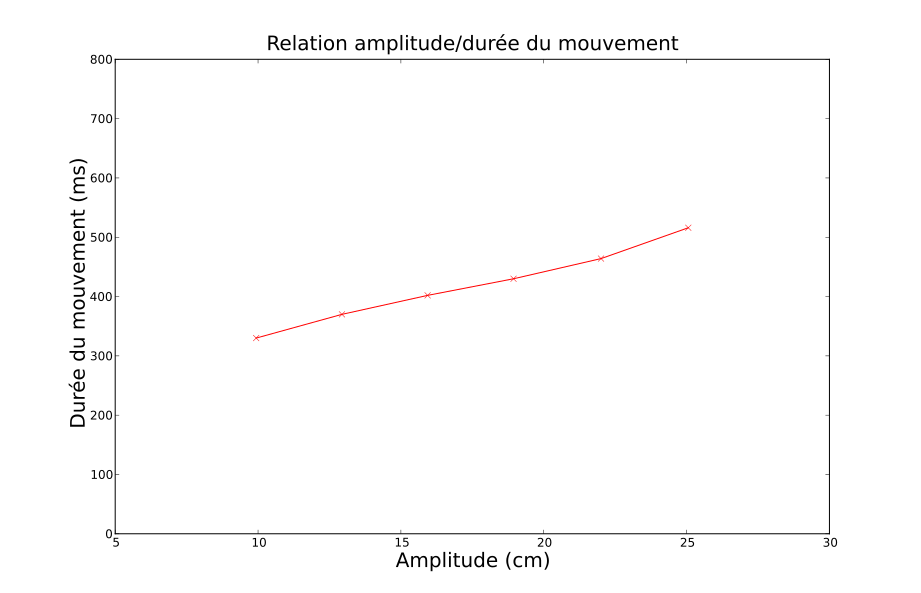
\includegraphics[width=.40\linewidth]{fig/lqp_scaling}}
%    \end{figure}
%    \begin{block}{Résultats}
%        $\qopslqp$ reproduit cette propriété
%    \end{block}
%\end{frame}
%
%\begin{frame}{Anisotropie}
%    \begin{itemize}
%        \item Propriété observée par $[$Gordon et al. 94$]$
%        \item Relation entre la durée du mouvement et sa direction
%    \end{itemize}
%    \begin{figure}
%        \centering
%        \subfigure{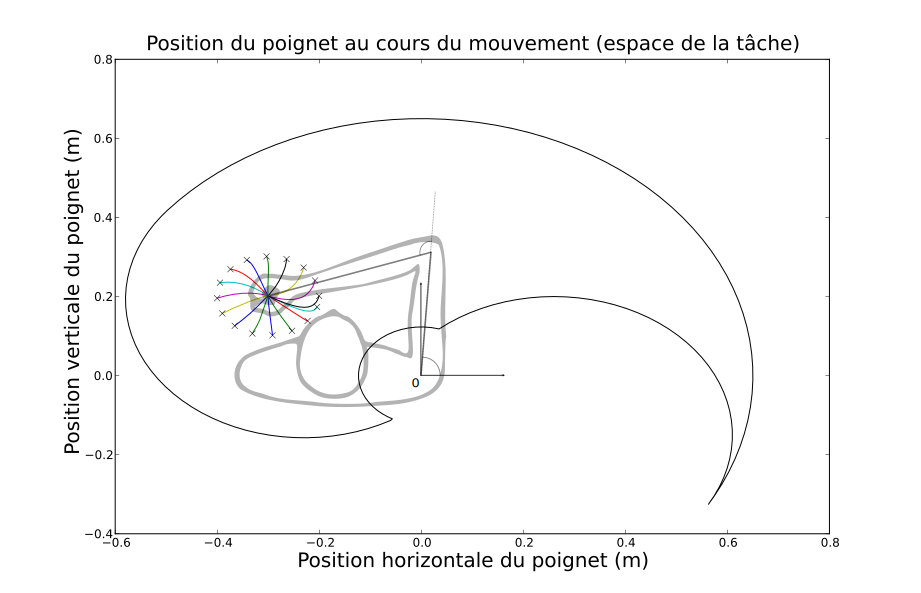
\includegraphics[width=.40\linewidth]{fig/lqp_anisotropie_paths_2}}~~~
%        \subfigure{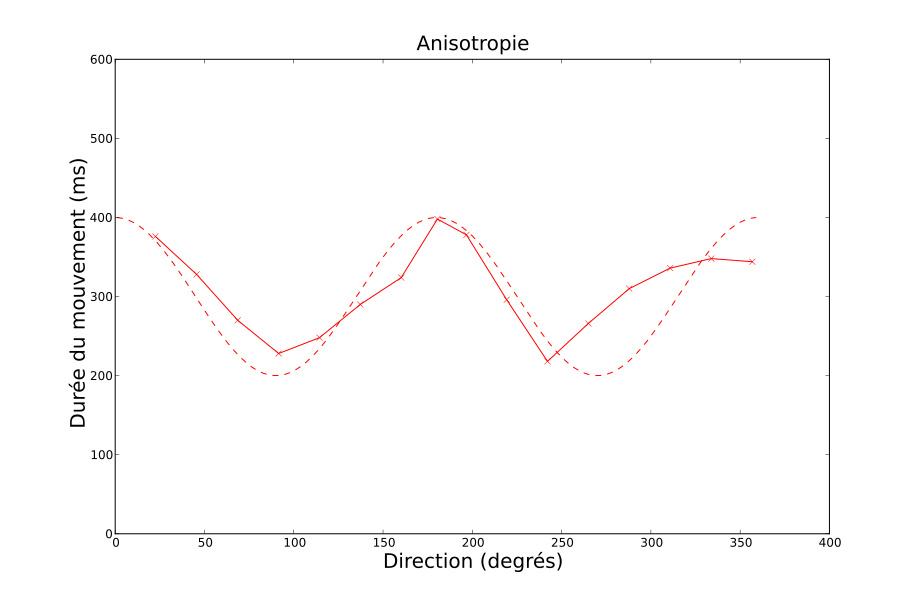
\includegraphics[width=.40\linewidth]{fig/lqp_anisotropy_2}}
%    \end{figure}
%    \begin{block}{Résultats}
%        $\qopslqp$ reproduit cette propriété
%    \end{block}
%\end{frame}

\begin{frame}{Loi de Fitts}
    \begin{small}
        \begin{itemize}
            \item Propriété observée par $[$Fitts 54$]$
            \item Relation entre la durée du mouvement et son indice de difficulté
        \end{itemize}
    \end{small}
    \begin{center}
        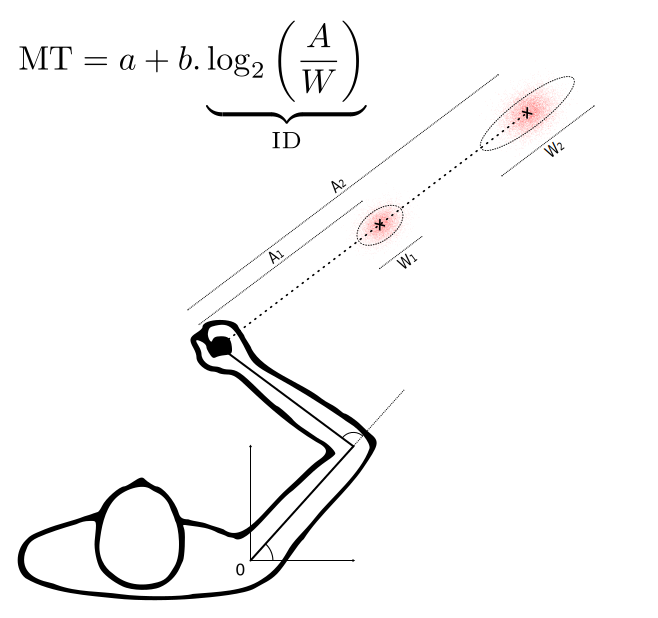
\includegraphics[width=.55\linewidth]{fig/fitts_exp2}
    \end{center}
\end{frame}

\begin{frame}{Loi de Fitts}
    \begin{figure}
        \centering
        \subfigure{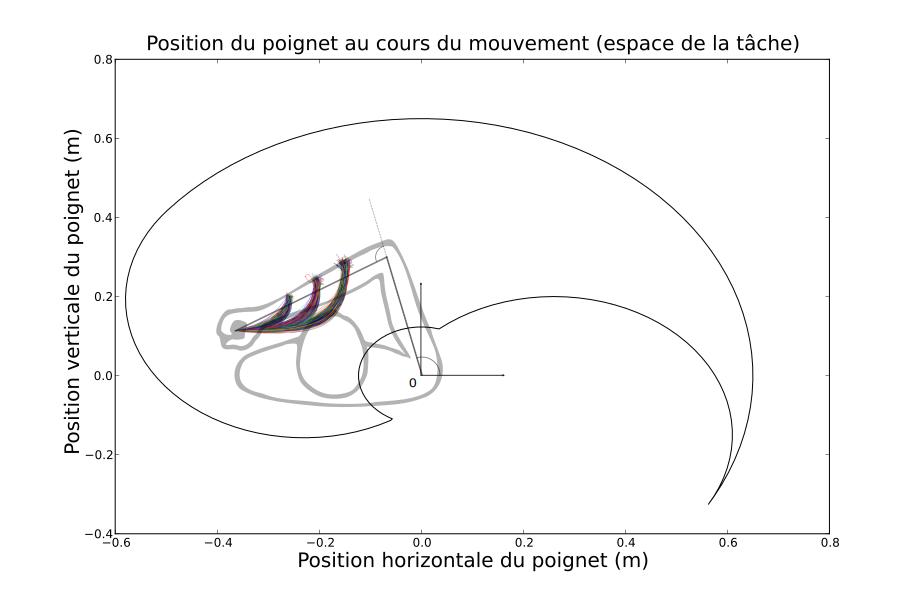
\includegraphics[width=.40\linewidth]{fig/lqp_fitts_paths_light2}}~~~
        \subfigure{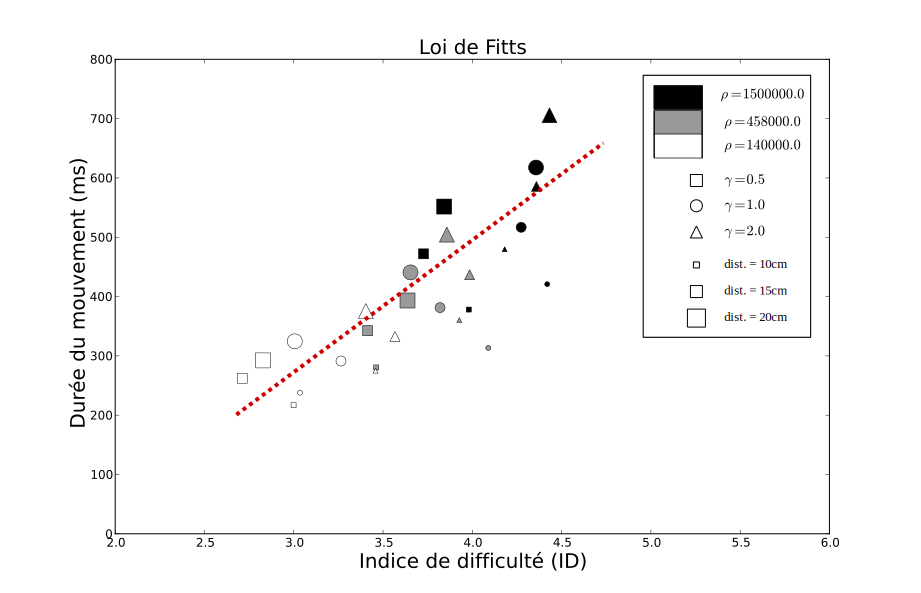
\includegraphics[width=.40\linewidth]{fig/lqp_fitts2_sigma4_2}}
    \end{figure}
    \begin{block}{Résultats}
        $\qopslqp$ reproduit cette propriété
    \end{block}
\end{frame}

\begin{frame}{Profil de variabilité}
    \begin{small}
        \begin{itemize}
            \item Propriété observée par $[$Selen et al. 06$]$
            \item Variabilité maximale en milieu de mouvement, minimale à la fin
        \end{itemize}
    \end{small}
    \begin{center}
        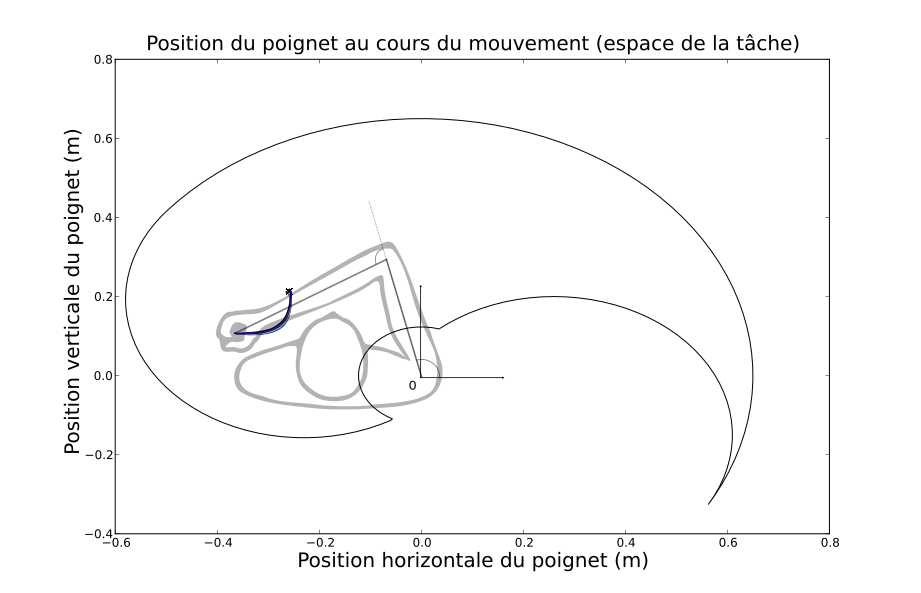
\includegraphics[width=.70\linewidth]{fig/lqp_variations_paths4}
    \end{center}
\end{frame}

\begin{frame}{Profil de variabilité}
    \begin{figure}
        \centering
        \subfigure[$\qopslqp$]{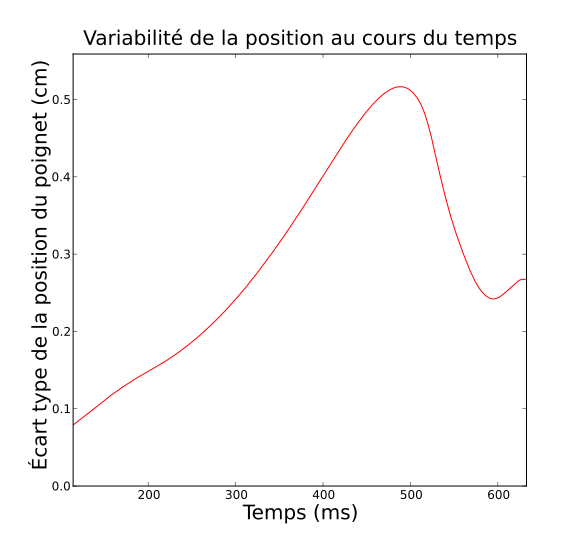
\includegraphics[width=.40\linewidth]{fig/variabilite}}~~~
        \subfigure[Selen et al. 06]{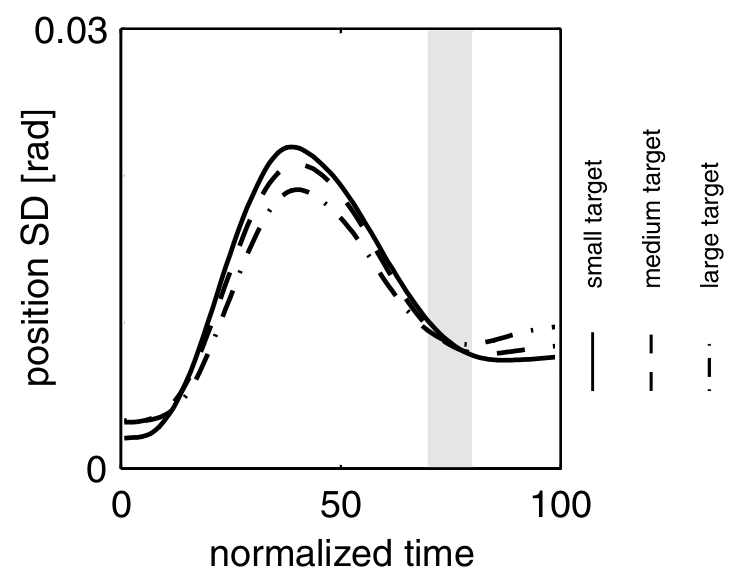
\includegraphics[width=.40\linewidth]{fig/selen06}}
    \end{figure}
    \begin{block}{Résultats}
        $\qopslqp$ reproduit cette propriété
    \end{block}
\end{frame}

